
%% Beginning of file == mru.tex ==
%% 
%% Created 23-07-2025
% Setting up the document class for Beamer
\documentclass{beamer}



% Configuring the Beamer theme
\usetheme{Madrid}
\usecolortheme{beaver}

%%%%%%%%%%%%%%%%%%%%%%%%%%%%%%%%%%%%%%%%%%%%%%%%%%%%%%%%%%%%
%% Paquetes.. %%%%%%%%%%%%%%%%%%%%%%%%%%%%%%%%%%%%%%%%%%%%%
%\usepackage[latin1]{inputenc}
% Including essential packages
\usepackage[utf8]{inputenc}
\usepackage[T1]{fontenc}
\usepackage{lmodern}
\usepackage{tikz} % For drawing the box with text
\usepackage{array} % For table formatting
\usepackage{cancel}
\usepackage{background}
\usepackage{amsmath}
\usetikzlibrary{arrows.meta, calc, shapes.geometric, backgrounds}


% Configuración del fondo pastel
%\backgroundsetup{
%    scale=1,
%    color=black,
%    opacity=0.8,
%    angle=0,
%    pages=all,
%    contents={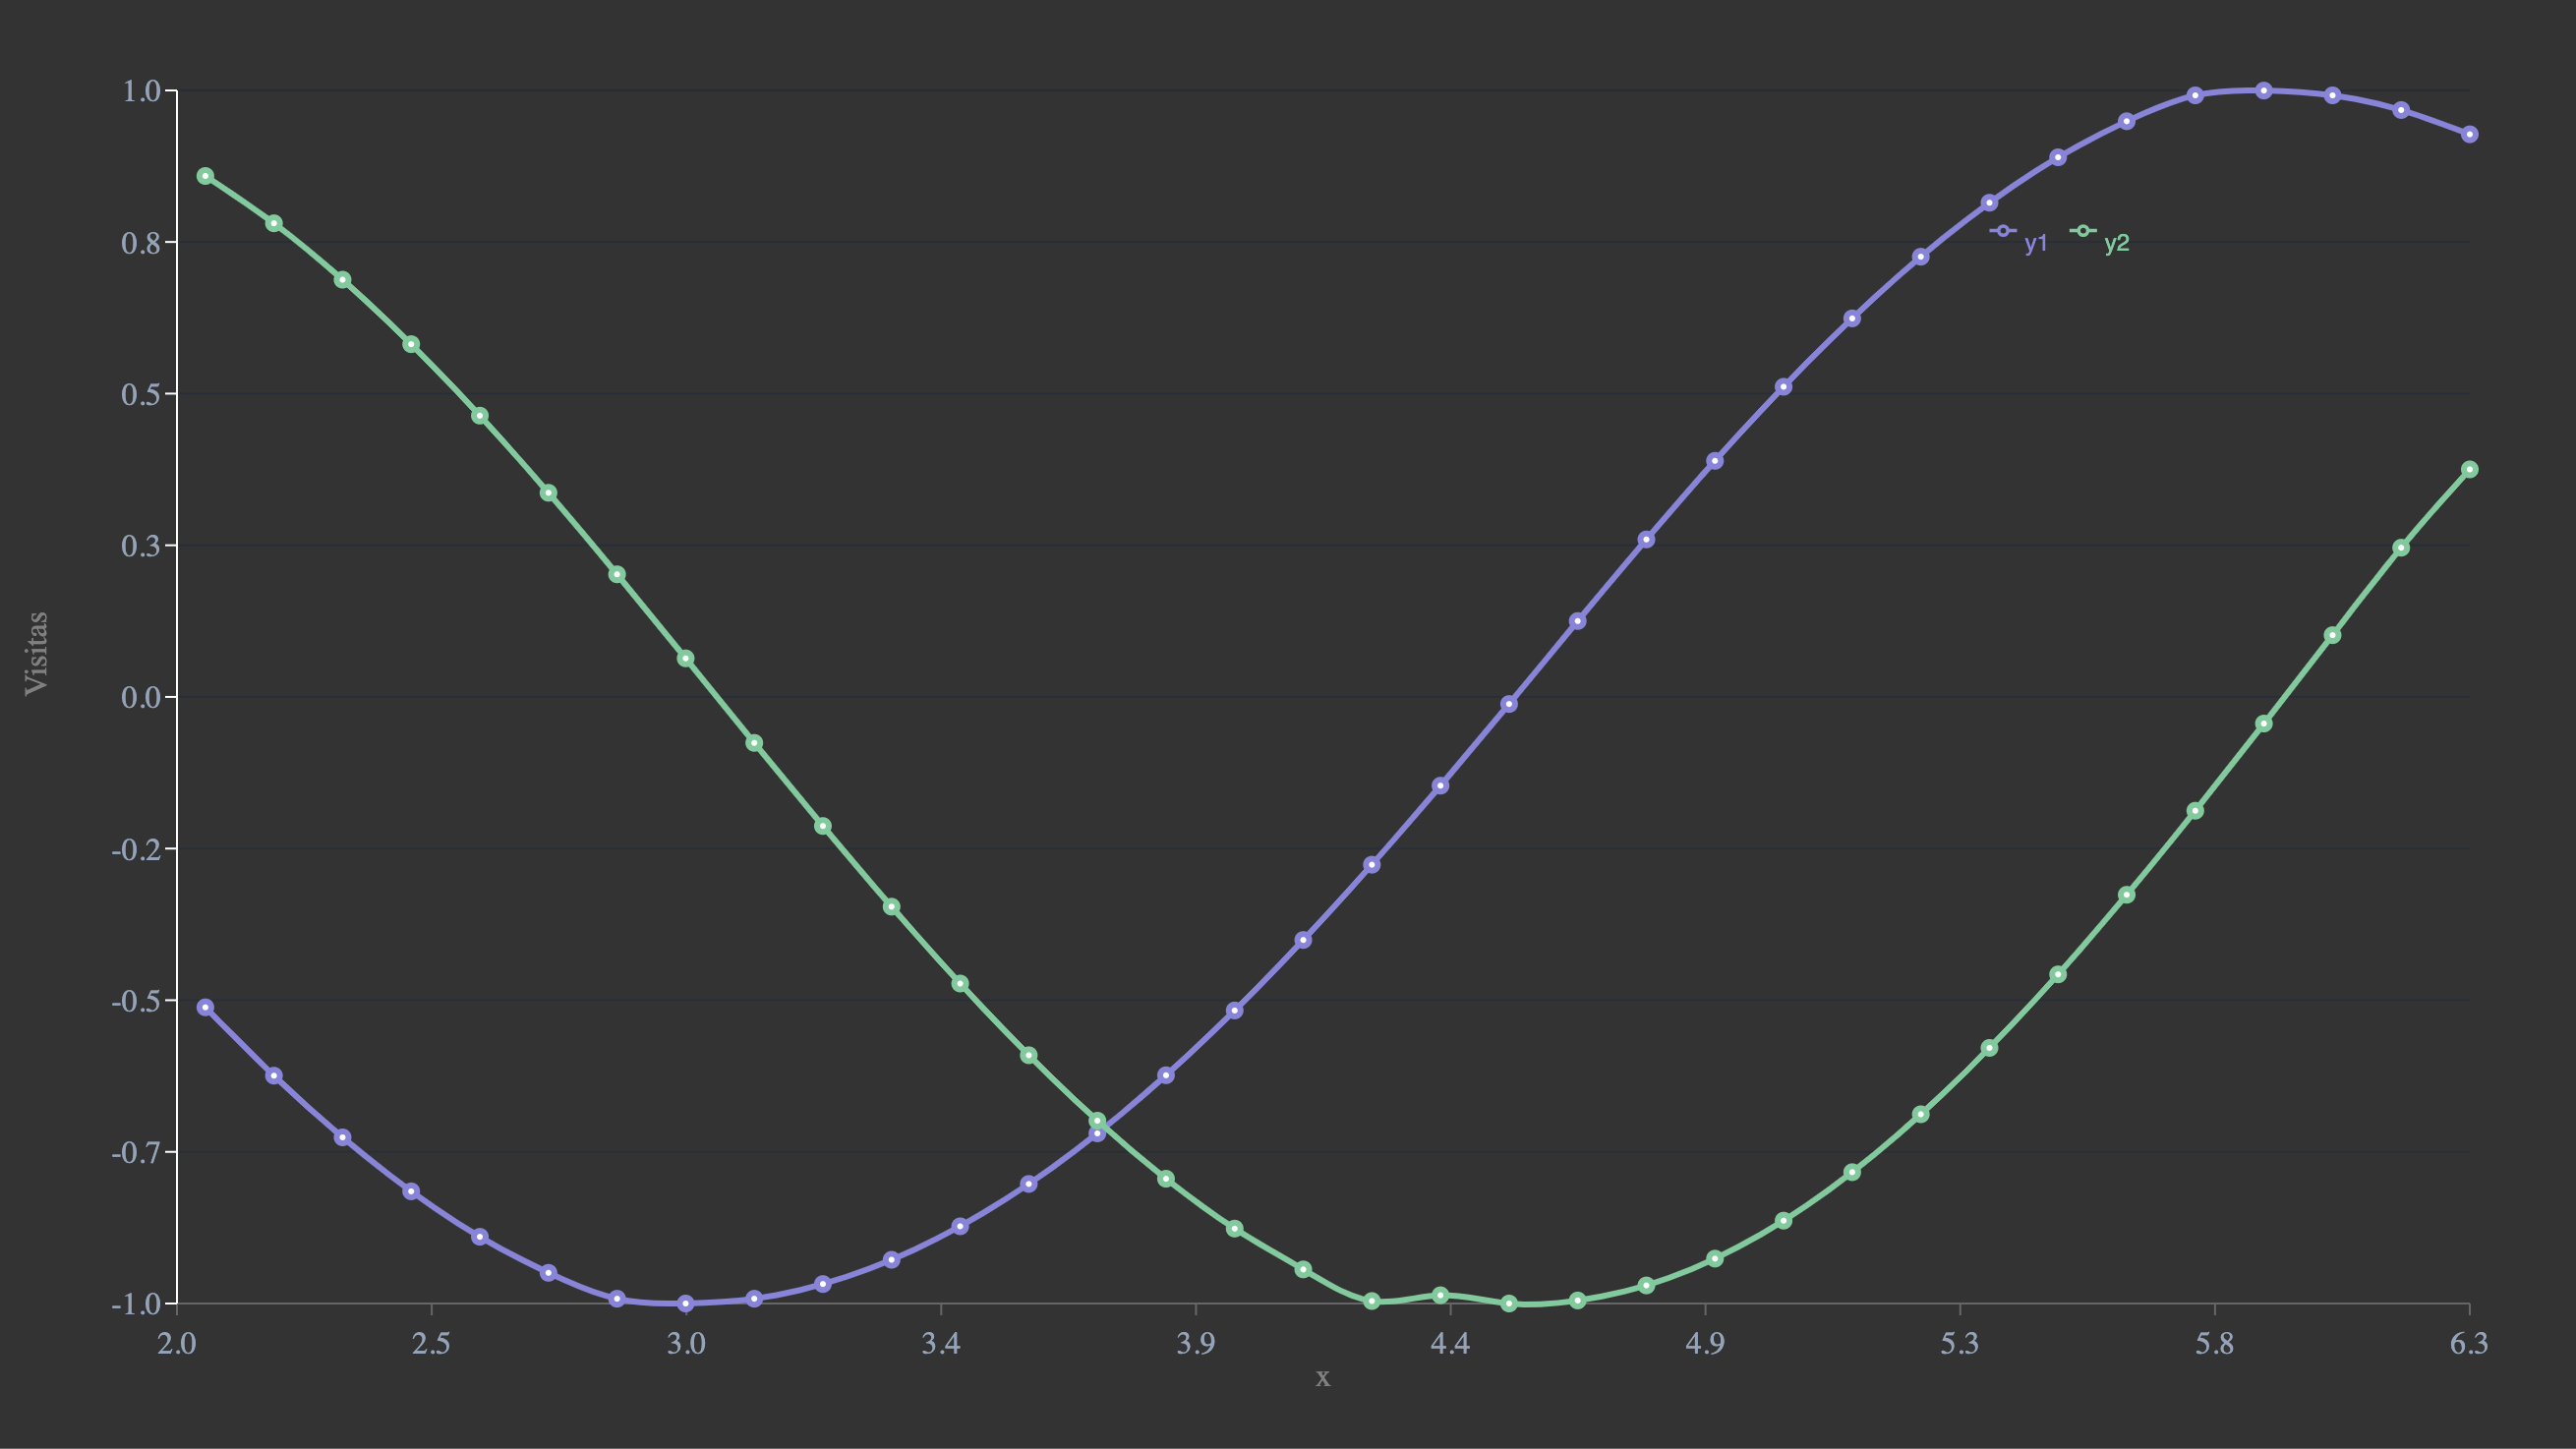
\includegraphics[width=\paperwidth,height=\paperheight]{images/imagen2.png}}
%}



%% You can insert definicions here..

%% DEFINICIONES MIAS..
%\def\psPiFour{12.566371}
%\def\psPiTwo{6.283185}
\def\psPi{3.14159265}
%\def\psPiH{1.570796327}
%\newdimen\pstRadUnit
%\newdimen\pstRadUnitInv
%\pstRadUnit=1.047198cm % this is pi/3
%\pstRadUnitInv=0.95493cm % this is 3/pi


%% Libreria de formulas %%%%%%%%%%%%%%%%%%%%%%%%%%%%%%%%%%%%
%% Velocidad en el Mov. Rec. Uniforme %%%%%%%%%%%%%%
\def\vmru{
%% Eq. 1 %%%%%%%%%%%%%
\begin{equation}
v=\frac{x}{t}
\label{vmru}
\end{equation}
%%%%%%%%%%%%%%%%%%%%%%%%%%%%%%%%%%%%%%%%%%%%%%%%%%%%
}

%% Distancia en el Mov. Rec. Uniforme %%%%%%%%%%%%%%
\def\xmru{
%% Eq. 2 %%%%%%%%%%%%%
\begin{equation}
x=vt
\label{xmru}
\end{equation}
%%%%%%%%%%%%%%%%%%%%%%%%%%%%%%%%%%%%%%%%%%%%%%%%%%%%
}

%% Tiempo en el Mov. Rec. Uniforme %%%%%%%%%%%%%%%%%
\def\tmru{
%% Eq. 3 %%%%%%%%%%%%%
\begin{equation}
t=\frac{x}{v}
\label{tmru}
\end{equation}
%%%%%%%%%%%%%%%%%%%%%%%%%%%%%%%%%%%%%%%%%%%%%%%%%%%%
}

%% Libreria de Notas    %%%%%%%%%%%%%%%%%%%%%%%%%%%%%%%%%%%%
%%%%%%%%%%%%%%%%%%%%%%%%%%%%%%%%%%%%%%%%%%%%%%%%%%%%
%%%%%%%%%%% NU para la velocidad %%%%%%%%%%%%%%%%%%%
%%%%%%%%%%%%%%%%%%%%%%%%%%%%%%%%%%%%%%%%%%%%%%%%%%%%
\def\vNUa%
{
%% Dibuja una cajita!! %%%%%%%%%%%%%%%%%%%
%% el background de gris..
\psframebox[linewidth=2pt,framearc=.3,fillstyle=solid,
fillcolor=lightgray]{
\begin{tabular}{c}
%%%%%%%%%%%%%%%%%%%%%%%%%%%%%%%%%%%%%%%%%%
{\bf Notas de Unidades}\\
{\sc magnitud}: Velocidad [v].
La velocidad puede venir en: \\

$\frac{{\rm km}}{{\rm h}}$ ; 
$\frac{{\rm m}}{{\rm s}}$ ; 
$\frac{{\rm cm}}{{\rm s}}$. \\

$1~\frac{{\rm km}}{{\rm h}}=
\frac{1000}{3600}~\frac{{\rm m}}{{\rm s}}
=\cancelto{0.277}{\frac{1}{3.6}}\frac{{\rm m}}{{\rm s}}$ \\

$1~\frac{{\rm m}}{{\rm s}} = 100~\frac{{\rm cm}}{{\rm s}}$

%%%%%%%%%%%%%%%%%%%%%%%%%%%%%%%%%%%%%%%%%%
\end{tabular}
}
%%%%%%%%%%%%%%%%%%%%%%%%%%%%%%%%%%%%%%%%%%

%% fin definicion de vNUa
}
%%%%%%%%%%%%%%%%%%%%%%%%%%%%%%%%%%%%%%%%%%%%%%%%%%%%
%%%%%%%%%%%%%%%%%%%%%%%%%%%%%%%%%%%%%%%%%%%%%%%%%%%%
%%%%%%%%%%%%%%%%%%%%%%%%%%%%%%%%%%%%%%%%%%%%%%%%%%%%

%%%%%%%%%%%%%%%%%%%%%%%%%%%%%%%%%%%%%%%%%%%%%%%%%%%%%%%%%%%%


%% Titulo y autor .. obligatorio..
\title{MRU i1: ver1}
\subtitle{Otoño - 2025}
\author{JM~Ramirez}
\date{\today}


%%%%%%%%%%%%%%%%%%%%%%%%%%%%%%%%%%%
%%% Comienzo del documento.. %%%%%%
%%%%%%%%%%%%%%%%%%%%%%%%%%%%%%%%%%%
\begin{document}
\maketitle
%%%%%%%%%%%%%%%%%%%%%%%%%%%%%%%%%%%

%%%%%%% Para pegar el log.. %%%%%%%%%%%%%%%%%%%%%%%%%%%%%%%
\logo{%
    \begin{tikzpicture}
        \node[opacity=0.2] {
\includegraphics[width=1cm]{images/citlogogrey.eps}};
    \end{tikzpicture}
}
%%%%%%%%%%%%%%%%%%%%%%%%%%%%%%%%%%%%%%%%%%%%%%%%%%%%%%%%%%%


%%%%%%% Advertencia para no dejar que se copien %%%%%%%%%%%
\addtobeamertemplate{footnote}{}{\gray \large Esta nota tiene la intenci\'on de que \'este material no sea entregado como tarea.}
%%%%%%%%%%%%%%%%%%%%%%%%%%%%%%%%%%%%%%%%%%%%%%%%%%%%%%%%%%%





%________________________________________________________________(ult. col, 65)
% ========================== slide1 ============================= 
\begin{frame}{Movimiento Rectil\'ineo Uniforme}
% 
% -Paragraph1 
%----------------------------------------------------------------
%----------------------------------------------------------------
% -Idea1 
% ============================================================== 
 La f\'ormula principal:

                                                               
% ============================================================== 
% -Idea2 
% ============================================================== 
 
{\huge \vmru}
\vNUa
                                                               
% ============================================================== 
% -Idea3 
% ============================================================== 
                                                               
                                                               
                                                               
% ============================================================== 
%----------------------------------------------------------------
%----------------------------------------------------------------
\end{frame}


%________________________________________________________________(ult. col, 65)
% ========================== slide2 ============================= 
\begin{frame}{MRU}
% 
% -Paragraph1 
%----------------------------------------------------------------
%----------------------------------------------------------------
% -Idea1 
% ============================================================== 

Recu\'erdalo por sus unidades:

% ============================================================== 
% -Idea2 
% ============================================================== 

\begin{equation*}
10\frac{\text{km}}{\text{h}} =
\frac{\text{Se recorren 10 km ({distancia})}}
{\text{en 1 hora ({tiempo})}}
\end{equation*}
                                                               
% ============================================================== 
% -Idea3 
% ============================================================== 
 
Las otras dos f\'ormulas que se derivan de (\ref{vmru}) son:

{\large \xmru \ \tmru}
                                                              
% ============================================================== 
%----------------------------------------------------------------
%----------------------------------------------------------------
\end{frame}


% ========================== slide3 ============================= 
\begin{frame}{MRU}
% 
% -Paragraph1 
%----------------------------------------------------------------
%----------------------------------------------------------------
% -Idea1 
% ============================================================== 
                                                               
Es uniforme porque la velocidad no var\'ia en el tiempo; \
(v es el mismo en cada unidad de tiempo!)
                                              
% ============================================================== 
% -Idea2 
% ============================================================== 
 
%%%%%%%%%%%%%%%%%%%%%%%%%%%%%
%% Para centrar el grafico %%
\begin{centering}
%%%%%%%%%%%%%%%%%%%%%%%%%%%%%
%%%%%%%%%%%%%%%%%%%%%%%%%%%%%

%% Propiedades del grafico.. %%%
%% el eje de X comienza aqui..
\def\iX{0.} %%
\def\iY{0.} %%
%% el eje de y comienza aqui..
\def\jX{8.5} %%
\def\jY{4.5} %%

%%%%%%%%%%%%%%%%%%%%%%%%%%%%%%%%%%%%%%%%%%%%%%%%%%%%%%%%%%%%%%
%% Este es el pspicture enviroment.. el mas sencillo %%%%%%%%%
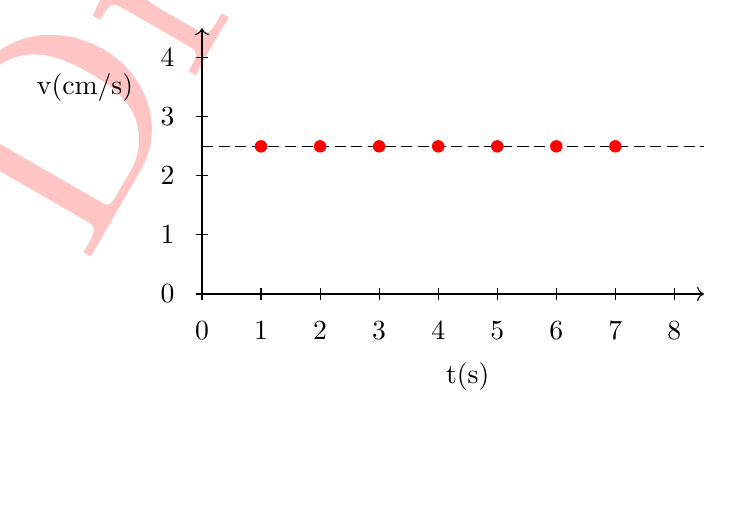
\begin{tikzpicture}[scale=0.75]
\path (-0.5,-3.5) rectangle (8.5,4.5); % Optional bounding box
% Axes
\draw[->] (0,0) -- (8.5,0);
\foreach \x in {0,1,...,8} {
  \draw (\x cm, 3pt) -- (\x cm, -3pt);
  \node[below] at (\x, -0.3) {\x};
}
\draw[->] (0,0) -- (0,4.5);
\foreach \y in {0,1,...,4} {
  \draw (3pt, \y cm) -- (-3pt, \y cm);
  \node[left] at (-0.3,\y) {\y};
}
\node[anchor=north] at (4.5,-1){t(s)};        %% Eje X
\node[anchor=east] at (-1,3.5){v(cm/s)};     %% Eje Y

%% Un recta y=ctte .. %%%%%%%
\def\iVctte{2.5}
%% (x1 , y1  )(x2 , y2=y1)
\draw[dashed, dash pattern=on 4pt off 2pt] (0,\iVctte) -- (8.5,\iVctte);
%%%%%%%%%%%%%%%%%%%%%%%%%%%%%%%%%%%%%%%%%%%%%%%%%%%%%
%%% El do de latex-pstricks!!! %%%%%%%%%%%%%%%%%%%%%%
%%% quiero poner unos punto rojos sobre la recta %%%%
\foreach \iA in {1,...,7}{
\fill[red] (\iA,\iVctte) circle[radius=3pt];}%
%%%%%%%%%%%%%%%%%%%%%%%%%%%%%%%%%%%%%%%%%%%%%%%%%%%%%
%%%%%%%%%%%%%%%%%%%%%%%%%%%%%%%%%%%%%%%%%%%%%%%%%%%%%                                                              
 
%%%%%%%%%%%%%%%%%%%%%%%%%%%%%%%%%%%%%
\end{tikzpicture}
%%%%%%%%%%%%%%%%%%%%%%%%%%%%%%%%%%%%%%%%%%%%%%%%%%%%%%%%%%%%%%
%%%%%%%%%%%%%%%%%%%%%%%%%%%%%%%%%%%%%%%%%%%%%%%%%%%%%%%%%%%%%%

%%%%%%%%%%%%%%%%%%%%%%%%%%%%%%
%% fin centrado del grafico %%
\end{centering}
%%%%%%%%%%%%%%%%%%%%%%%%%%%%%%
%%%%%%%%%%%%%%%%%%%%%%%%%%%%%%
                                                              
                                                               
% ============================================================== 
% -Idea3 
% ============================================================== 
                                                               
                                                               
                                                               
% ============================================================== 
%----------------------------------------------------------------
%----------------------------------------------------------------
\end{frame}

%________________________________________________________________(ult. col, 65)


%________________________________________________________________(ult. col, 65)
% ========================== frame1 ============================= 
\begin{frame}{MRU}
% 
% -Paragraph1 
%----------------------------------------------------------------
%----------------------------------------------------------------
% -Idea1 
% ============================================================== 
 
Un << auto >> { anda } a { 152 km/h }. Comienza su pase por un puente y { 205 segundos } despu\'es est\'a en el otro extremo, saliendo completamente (del puente) { 15 segundos } despu\'es. ?`Cu\'al es la { longitud } del puente y cu\'al es la longitud del << auto >>? %% Hay 0 elementos de distancia %% Hay 2 elementos de tiempo %% Hay 1 elementos de velocidad


% ============================================================== 
% -Idea2 
% ============================================================== 
 
\begin{itemize}                                                              

\item El 1er paso en la resoluci\'on de cualquier problema, es la
identificaci\'on de los elementos del problema.            
              
\end{itemize}

% ============================================================== 
%----------------------------------------------------------------
%----------------------------------------------------------------
\end{frame}


%________________________________________________________________(ult. col, 65)
% ========================== slide1 ============================= 
\begin{frame}{MRU}
% 
% -Paragraph1 
%----------------------------------------------------------------
% ============================================================== 
% -Idea1 
% ============================================================== 
 
%% Dibuja una cajita!! %%%%%%%%%%%%%%%%%%%
%% el background de gris..
\begin{center}
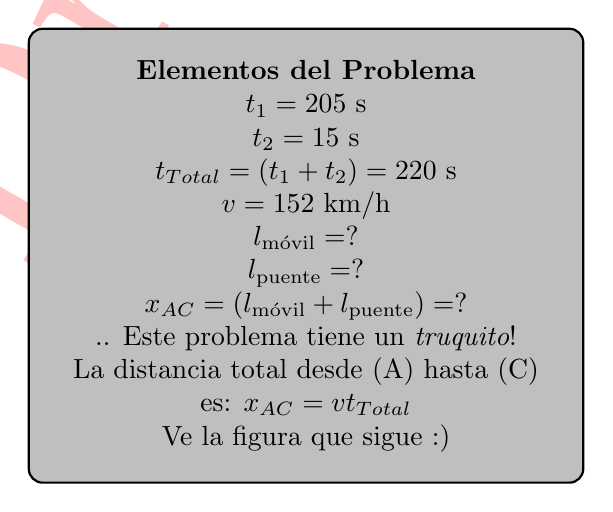
\begin{tikzpicture}
    \node[draw, line width=0.8pt, rounded corners=5pt, fill=lightgray, inner sep=10pt] (box) {
        \begin{tabular}{c}
%%%%%%%%%%%%%%%%%%%%%%%%%%%%%%%%%%%%%%%%%%

{\bf Elementos del Problema}\\
$t_{1}=205$ s  \\
$t_{2}=15$ s  \\
$t_{Total}=(t_{1}+t_{2})=220$ s  \\
$v=152$ km/h \\
$l_{\text{m\'ovil}}=?$   \\
$l_{\text{puente}}=?$ \\ 
$x_{AC}=(l_{\text{m\'ovil}}+l_{\text{puente}})=$? \\
    .. Este problema tiene un {\it truquito}! \\
    La distancia total desde (A) hasta (C) \\
    es: $x_{AC}=vt_{Total}$ \\
    Ve la figura que sigue :) 

%%%%%%%%%%%%%%%%%%%%%%%%%%%%%%%%%%%%%%%%%%
\end{tabular}
    };
\end{tikzpicture}
\end{center}

% Adding the small drawing with text below the box
\vspace{0.5cm}
\begin{center}
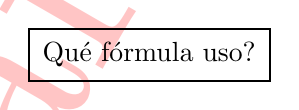
\begin{tikzpicture}
    \node[draw, line width=0.8pt, inner sep=5pt] at (0,0) {Qu\'e f\'ormula uso?};
\end{tikzpicture}
\end{center}

% ============================================================== 
%----------------------------------------------------------------
%----------------------------------------------------------------
\end{frame}


%________________________________________________________________(ult. col, 65)
% ========================== slide2 ============================= 
\begin{frame}{MRU}
% 
% -Paragraph1 
%----------------------------------------------------------------
%----------------------------------------------------------------
% -Idea1 
% ==============================================================

% Requires \usepackage{tikz} and \usetikzlibrary{arrows.meta} in the Beamer preamble
\begin{center}
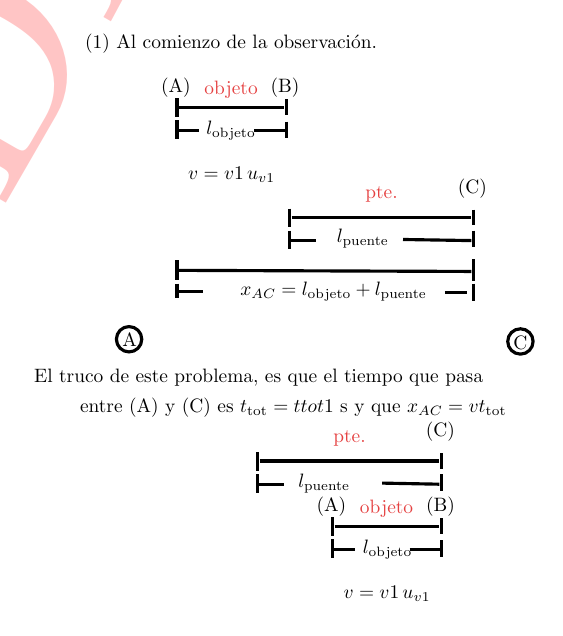
\begin{tikzpicture}[scale=0.7, transform shape]
    \definecolor{color934}{rgb}{0.8980392156862745,0.25882352941176473,0.25882352941176473}
    % First diagram
    \node at (5.66, 4.99) {(1) Al comienzo de la observaci\'{o}n.};
    \draw[line width=0.4mm] (4.72, 3.84) -- (6.62, 3.84);
    \draw[line width=0.4mm] (4.68, 4.00) -- (4.68, 3.66);
    \draw[line width=0.4mm] (6.66, 3.98) -- (6.66, 3.70);
    \draw[line width=0.4mm] (4.68, 3.60) -- (4.68, 3.26);
    \draw[line width=0.4mm] (4.68, 3.42) -- (5.08, 3.42);
    \draw[line width=0.4mm] (6.08, 3.42) -- (6.64, 3.42);
    \draw[line width=0.4mm] (6.66, 3.58) -- (6.66, 3.28);
    \node[color=color934] at (5.66, 4.15) {objeto};
    \node at (5.66, 3.41) {$l_{\text{objeto}}$};
    \node at (4.66, 4.19) {(A)};
    \node at (6.64, 4.19) {(B)};
    %\draw[line width=0.4mm, -{Stealth[length=1.4mm]}] (4.70, 2.92) -- (6.70, 2.90);
    \node at (5.67, 2.61) {$v=v1 \, u_{v1}$};
    % Second diagram
    \draw[line width=0.4mm] (6.76, 1.84) -- (10.02, 1.84);
    \draw[line width=0.4mm] (6.72, 2.00) -- (6.72, 1.66);
    \draw[line width=0.4mm] (10.06, 1.98) -- (10.06, 1.70);
    \draw[line width=0.4mm] (6.72, 1.60) -- (6.72, 1.26);
    \draw[line width=0.4mm] (6.72, 1.42) -- (7.20, 1.42);
    \draw[line width=0.4mm] (8.78, 1.44) -- (10.02, 1.42);
    \draw[line width=0.4mm] (10.06, 1.60) -- (10.06, 1.30);
    \node[color=color934] at (8.39, 2.25) {pte.};
    \node at (8.05, 1.45) {$l_{\text{puente}}$};
    \node at (10.04, 2.37) {(C)};
    % Third diagram
    \draw[line width=0.4mm] (4.68, 0.88) -- (10.02, 0.86);
    \draw[line width=0.4mm] (10.06, 1.08) -- (10.06, 0.68);
    \draw[line width=0.4mm] (4.68, 1.06) -- (4.68, 0.70);
    \draw[line width=0.4mm] (4.68, 0.64) -- (4.68, 0.38);
    \draw[line width=0.4mm] (4.72, 0.50) -- (5.16, 0.50);
    \draw[line width=0.4mm] (9.54, 0.48) -- (9.94, 0.48);
    \draw[line width=0.4mm] (10.06, 0.64) -- (10.06, 0.32);
    \node at (7.52, 0.49) {$x_{AC}=l_{\text{objeto}}+l_{\text{puente}}$};
    \draw[line width=0.4mm, fill=white] (3.81, -0.37) circle (0.23);
    \node at (3.82, -0.39) {A};
    %\draw[line width=0.4mm, -{Stealth[length=1.4mm]}] (4.00, -0.14) -- (4.60, 0.42);
    \draw[line width=0.4mm, fill=white] (10.91, -0.41) circle (0.23);
    \node at (10.91, -0.43) {C};
    %\draw[line width=0.4mm, -{Stealth[length=1.4mm]}] (10.64, -0.26) -- (10.24, 0.26);
    % Fourth diagram
    \draw[line width=0.4mm] (6.18, -2.58) -- (9.44, -2.58);
    \draw[line width=0.4mm] (6.14, -2.42) -- (6.14, -2.76);
    \draw[line width=0.4mm] (9.48, -2.44) -- (9.48, -2.72);
    \draw[line width=0.4mm] (6.14, -2.82) -- (6.14, -3.16);
    \draw[line width=0.4mm] (6.14, -3.00) -- (6.62, -3.00);
    \draw[line width=0.4mm] (8.40, -2.98) -- (9.44, -3.00);
    \draw[line width=0.4mm] (9.48, -2.82) -- (9.48, -3.12);
    \node[color=color934] at (7.81, -2.17) {pte.};
    \node at (7.35, -2.99) {$l_{\text{puente}}$};
    \node at (9.46, -2.05) {(C)};
    % Fifth diagram
    \draw[line width=0.4mm] (7.54, -3.76) -- (9.44, -3.76);
    \draw[line width=0.4mm] (7.50, -3.60) -- (7.50, -3.94);
    \draw[line width=0.4mm] (9.48, -3.62) -- (9.48, -3.90);
    \draw[line width=0.4mm] (7.50, -4.00) -- (7.50, -4.34);
    \draw[line width=0.4mm] (7.50, -4.18) -- (7.90, -4.18);
    \draw[line width=0.4mm] (8.90, -4.18) -- (9.46, -4.18);
    \draw[line width=0.4mm] (9.48, -4.02) -- (9.48, -4.32);
    \node[color=color934] at (8.48, -3.45) {objeto};
    \node at (8.50, -4.19) {$l_{\text{objeto}}$};
    \node at (7.48, -3.41) {(A)};
    \node at (9.46, -3.41) {(B)};
    %\draw[line width=0.4mm, -{Stealth[length=1.4mm]}] (7.52, -4.68) -- (9.52, -4.70);
    \node at (8.49, -4.99) {$v=v1 \, u_{v1}$};
    % Text annotations
    \node at (6.16, -1.07) {El truco de este problema, es que el tiempo que pasa};
    \node at (6.79, -1.61) {entre (A) y (C) es $t_{\text{tot}}=ttot1$ s y que $x_{AC}=v t_{\text{tot}}$};
\end{tikzpicture}
\end{center}


% ============================================================== 
%----------------------------------------------------------------
%----------------------------------------------------------------
\end{frame}


%________________________________________________________________(ult. col, 65)
% ========================== frame2 ============================= 
\begin{frame}{MRU}
% 
% -Paragraph1 
%----------------------------------------------------------------
%----------------------------------------------------------------
% -Idea1 
% ============================================================== 
 
{\huge                
\xmru
}                                             
 
% ============================================================== 
% -Idea2 
% ============================================================== 

%%%%%%%%%%%%%%%%%%%%%%%%%%%%%%%%%%%%%%%%%%%%%%%%%%%%%%%%%%%%%%%%
%%%%%%%%%%%%%%%%% Cajita de Texto sencilla %%%%%%%%%%%%%%%%%%%%%
\begin{center}
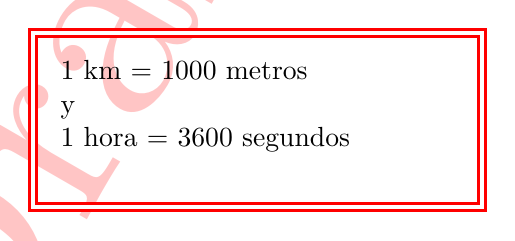
\begin{tikzpicture}
    % Creating a double-framed box with red border
    \node[
        draw=red, 
        line width=0.42mm, % Approximating 1.5pt
        double, 
        double distance=0.5mm, % Simulating psdblframebox
        inner sep=10pt
    ] (box) {
        \parbox[c]{5cm}{
1 km =  1000 metros \\
y \\
1 hora =  3600 segundos \\

        }
    };
\end{tikzpicture}
\end{center}
%%%%%%%%%%%%%%%%%%%%%%%%%%%%%%%%%%%%%%%%%%%%%%%%%%%%%%%%%%%%%%%%
%%%%%%%%%%%%%%%%%%%%%%%%%%%%%%%%%%%%%%%%%%%%%%%%%%%%%%%%%%%%%%%%
                           
% ============================================================== 
% -Idea3 
% ============================================================== 
 
Finalmente..                                                              
                                                               
                                                               
% ============================================================== 
%----------------------------------------------------------------
%----------------------------------------------------------------
\end{frame}


%________________________________________________________________(ult. col, 65)
% ========================== frame3 ============================= 
\begin{frame}{MRU}
% 
% -Paragraph1 
%----------------------------------------------------------------
% ============================================================== 
% -Idea1
% ==============================================================

La longitud del puente es:
{\large
\begin{equation} 
l_{\text{puente}}=
152~(\frac{1000}{3600})~
\frac{m}{\cancel{s}}~[205~\cancel{s}]=
8655~m
\end{equation}
}

                               
% ============================================================== 
% -Idea2 
% ============================================================== 

La distancia total desde (A) a (C) es: 
{\large
\begin{equation} 
x_{AC}=
152~(\frac{1000}{3600})~
\frac{m}{\cancel{s}}~[220~\cancel{s}]=
9288~m
\end{equation}
}

% ============================================================== 
%----------------------------------------------------------------
%----------------------------------------------------------------
\end{frame}


%%%%%%%%%%%%%%%%%%%%%%%%%%%%%%%%%%%%%%%%%%%%%%%%%%%%%%
%%%%%%%%%%%%%%%  Tail  %%%%%%%%%%%%%%%%%%%%%%%%%%%%%%%
%%%%%%%%%%%%%%%%%%%%%%%%%%%%%%%%%%%%%%%%%%%%%%%%%%%%%%

\end{document}
%%
%% End of file == mru.tex ==
%%
%% Modified 23-07-2025 
